
\section{Method}

\subsection{Data collection}

\subsection{Filtering process}

\subsection{Integration Model}



\begin{frame}
  \frametitle{Previous Integration Model }
    Distance and Velocity Equations (Ballistic Integration):
\onslide<2, 3, 4>{
    \begin{align*}
        s(k+1) &= s(k) + dt \cdot v(k) + \frac{dt^2}{2} a(k) \\
        v(k+1) &= v(k) + dt \cdot a(k)
    \end{align*}

}
\onslide<3, 4>{

    \hfil

    Acceleration Equations (Rearranged):
    \begin{align*}
    From \ distance: \ \ \ \ \ \  a(k) &= \frac{2}{dt^2} \Bigl( s(k+1) - s(k) - dt \cdot v(k) \Bigr)\\
    From \ velocity: \ \ \ \ \ \ a(k) &= \frac{1}{dt} \Bigl( v(k+1) - v(k) \Bigr)
    \end{align*}
}
\onslide<4>{

\textbf{Problem:} Accelerations don't add up!

}
\end{frame}

\begin{frame}
    \frametitle{Previous Integration Model - Accuracy}
    \begin{figure}
        \centering
        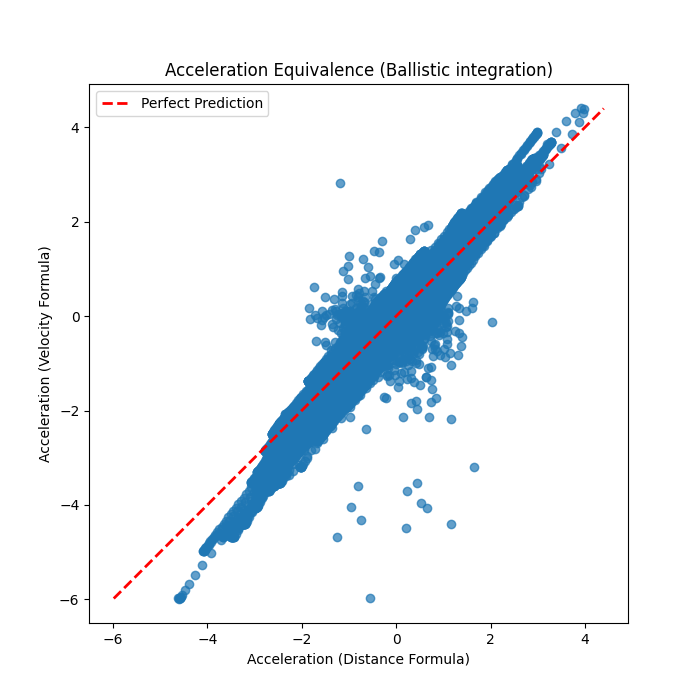
\includegraphics[width=0.65\textwidth]{figures/graphs/Acceleration Equivalence (Ballistic integration).png}
    \end{figure}
\end{frame}

\begin{frame}
  \frametitle{Our Integration Model}
    Our Distance and Velocity Equations:
\onslide<2, 3>{
    \begin{align*}
    s(t+1) &= s(t) + dt \cdot v(t)+ \textcolor{red}{c_1} a(t) + \textcolor{red}{c_2} a(t-1) \\
    v(t+1) &= v(t) + \textcolor{red}{c_3} a(t) + \textcolor{red}{c_4} a(t-1)
    \end{align*}

    \hfil
}
\onslide<3>{

    Our Acceleration Equations:
    \begin{align*}
    a(k) &= - \overline{\textcolor{red}{c_1}} a(k-1)  + \overline{\textcolor{red}{c_2}} \bigl( s(k+1) - s(k) - dt \cdot  v(k)\bigr)\\
    a(k) &= - \overline{\textcolor{red}{c_3}} a(k-1)  + \overline{\textcolor{red}{c_4}} \bigl( v(k+1) - v(k) \bigr) 
    \end{align*}
}
\end{frame}

\begin{frame}
  \frametitle{Our Integration Model - Matrix Form}
  \onslide<1->{
    Acceleration from Distance formula:
    \begin{align*}
        \begin{bmatrix} a(k-1) \\ \end{bmatrix}
        &=
        \begin{bmatrix}
            -a(k)  & v(k+1) - v(k)   \\ 
        \end{bmatrix}
        \begin{bmatrix}
            \overline{\textcolor{red}{c_1}} \\
            \overline{\textcolor{red}{c_2}} \\
        \end{bmatrix} \\
    \end{align*}

    Acceleration from Velocity formula:
    \begin{align*}
        \begin{bmatrix}
            a(k-1) \\ 
        \end{bmatrix}
        &=
        \begin{bmatrix}
            -a(k) &    s(k+1) - s(k) - dt \  v(k)   \\ 
        \end{bmatrix}
        \begin{bmatrix}
            \overline{\textcolor{red}{c_3}} \\
            \overline{\textcolor{red}{c_4}} \\
        \end{bmatrix}
    \end{align*}
  }

    \hfil

  \onslide<2->{
    $\Rightarrow$ This can be solved using linear regression.
  }
\end{frame}
